\section{Prüfung}
\textit{Haben Sie denn einen Lieblingsversuch.}
\\\\\noindent
Ja, den Photoeffekt.
\\\\\noindent
\textit{Dann erzählen Sie uns doch mal etwas dazu. Wir kennen den Versuch beide nicht.}
\\\\\noindent
Unter dem Photoeffekt versteht man das Auslösen von Elektronen aus einer Metalloberfläche durch die Bestrahlung mit Licht. Das Spannende
an dem Versuch ist dabei, dass er nur mit dem Korpuskelmodell erklärt werden kann. Bis dahin wurde Licht als Welle verstanden, was sowohl
die Elektrodynamik als auch Versuche wie der Doppelspalt stützen.
\\\\\noindent
Ich denke, ich skizziere erst einmal den Versuchsaufbau und erkläre dann das Prinzip der Messung.
\begin{figure}[H]
    \centering
    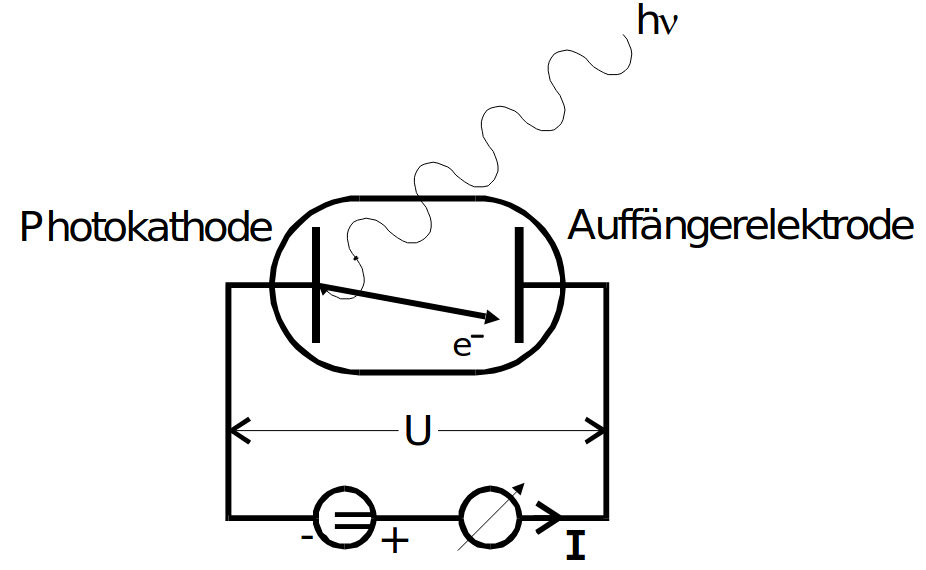
\includegraphics[scale=0.4]{pictures/Anordnung1.png}
    \caption{Versuchsaufbau der Gegenfeldmethode. \cite{AP01}}
    \label{fig:Gegenfeld}
\end{figure}
\noindent 
(Es folgt eine Erklärung der Gegenfeldmethode nach Abbildung \ref{fig:Gegenfeld}). 
Dabei sind 4 Beobachtungen zu machen:
\begin{enumerate}
    \item Die Energie des Elektrons ist proportinal zur Frequenz und insbesondere nicht abhängig von der Intensität des Lichts, wie es beim 
        Wellenmodell zu erwarten wäre. 
    \item Daraus folgt im Prinzip direkt, dass es eine Grenzfrequenz gibt, unter der der Photoeffekt nicht mehr auftreten kann.
    \item Jetzt kommt doch die Intensität ins Spiel, denn eine Vergrößerung der Lichtintensität sorgt für einen größeren Photostrom. 
        Das bedeutet aber nur, dass dann mehr Elektronen ausgelöst werden. Die Energie der Elektrons ändert sich dabei nicht.
    \item Der vierte Punkt wirkt recht trivial. Es geht draum, dass der Photoeffekt beinahe direkt mit der Lichtbestrahlung anfängt
        und auch direkt wieder aufhört, wenn man die Lampe ausschaltet. Bei einer Welle bräuchte man ja eine gewisse Anregungszeit. Die 
        haben wir hier nicht.
\end{enumerate}
Den Zusammenhang zwischen der Energie der Elektronen und der Frequenz des Lichts bekommen wir durch das Aufstellen der Energiebilanz 
(Abb.\ref{fig:Energiebilanz}). 
\begin{figure}[H]
    \centering
    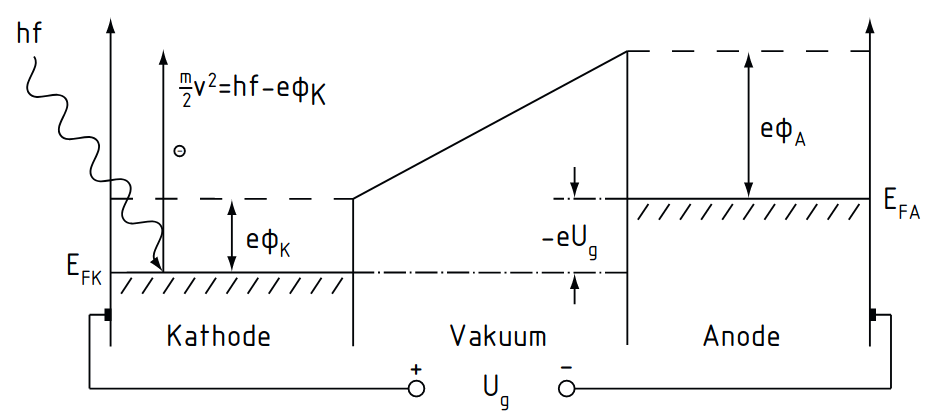
\includegraphics[scale=0.4]{pictures/Energiebilanz.png}
    \caption{Energiebilanz. \cite{AP02}}
    \label{fig:Energiebilanz}
\end{figure}
\noindent 
Da haben wir erst die Ferminiveaus der beiden Elektroden. Durch Anlegen der Gegenspannung verschiebt sich die Energie der Anode noch weiter
nach oben. Jetzt haben Anode und Kathode unterschiedliche Austrittsarbeiten. Die Kathode besteht aus Cäsium und besitzt eine sehr niedrige 
Austrittsarbeit, die der Anode ist deutlich größer. Und jetzt sieht man auch schon direkt den Potentialberg, den das Elektron überwinden muss.
Dafür benötigt es dann die Differenz nach oben als kinetische Energie. Wenn ein Photon also ein Elektron aus dem Ferminiveau trifft, muss es 
dann genau diese Energie hier besitzen, damit das Elektron dann gerade so an der Anode ankommt. Hier sieht man auch nochmal ganz schön, wie 
man die Messung durchführt. Wir variieren die Spannung, heben und senken also die Energie der Anode. Bei einer Grenzspannung reicht das 
Photon dann grade nicht mehr aus, um dem Elektron genung Energie zu geben um zur Anode zu gelangen. Und das kann man dann mit mehreren Frequenzen 
des Lichts machen, die wir mit einem Prisma aus einer Quecksilber-Dampflampe gewinnen. Aus dieser Energiebilanz kann man jetzt auch direkt 
2 Zusammenhänge ablesen:
\begin{align}
    h\nu&=E_{kin}+\Phi_K \\
    h\nu&=e_0U_{g,max}+\Phi_A \label{eqn:Einstein}
\end{align}
In der Anleitung sah die Formel anders aus. Da hatten wir die untere, aber anstatt der Austrittsarbeit der Anode, stand da die der Kathode. 
Diese misst man dann tatsächlich auch eher. Das liegt vor allem daran, dass Cäsium verdampft und sich dann kleine Partikel auf die Anode 
setzten. Diese sind ja für die anfliegenden Elektronen Potentialminima, da sie das Kontaktpotential absenken. 
Soll ich weiter machen? 
\\\\\noindent
\textit{Gerne}
\\\\\noindent
Das Problem ist jetzt, dass der Photostrom nicht direkt verschwindet. Die Energiebilanz stimmt nämlich nur für eine scharfe Fermikante. 
Diese weicht aber bei höhreren Temperaturen auf, sodass wir bei Raumtemperatur dann schnellere und langsamere Elektronen in der Kathode finden
(Abb.\ref{fig:Fermi}). 
\begin{figure}[H]
    \centering
    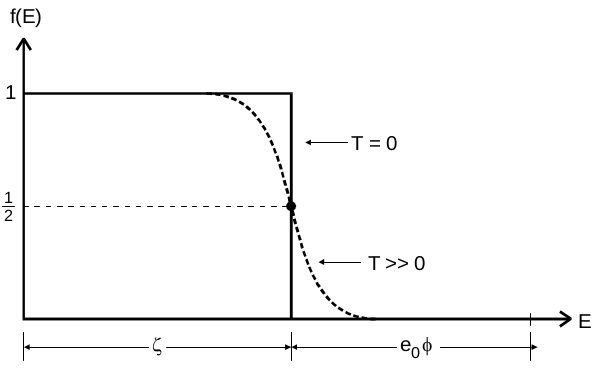
\includegraphics[scale=0.5]{pictures/fermidirac.png}
    \caption{Fermi-Dirac-Verteilung. \cite{AP03}}
    \label{fig:Fermi}
\end{figure}
\noindent
Man kann sich das dann so vorstellen, dass zuerst die langsamen Elektronen nicht mehr gegen das Gegenfeld ankommen 
und der Strom dann allmählich abnimmt, bis auch die schnellen Elektronen die Anode nicht mehr errreichen (Abb.\ref{fig:U-I}). Da ist es dann
sehr schwierig die Grenzspannung zu ermitteln. 
\begin{figure}[H]
    \centering
    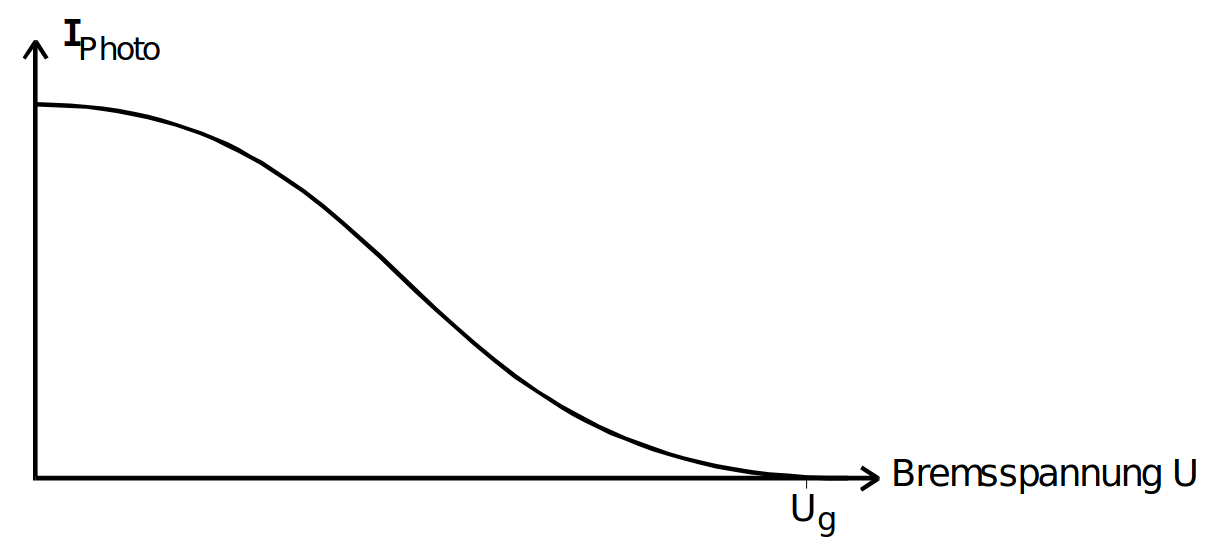
\includegraphics[scale=0.4]{pictures/Photostrom.png}
    \caption{$U_G-I_P$-Diagramm. \cite{AP01}}
    \label{fig:U-I}
\end{figure}
\noindent 
Man kann aber zeigen, dass $U_{g}^2\propto I_{P}$ ist, sodass wir bei einem 
$(U_g-\sqrt{I_P})$-Diagramm einen linearen Verlauf sehen und die Grenzfrequenz dann einfach als Nullstelle ablesen. Wenn man das dann für 
mehrere Frequenzen gemacht hat, kann man die Werte noch in ein $(\nu-U_{g,max})$-Diagramm eintragen. Das ist dann genau die umgestellte Formel 
\ref{eqn:Einstein}, womit die Steigung der Geraden dann das Planksche Wirkungsquantum ist. Die Diskussion des y-Abschnitts ist jedoch ein 
wenig schwieriger, da die Austrittsarbeit der Anode ja dem Störeffekt unterliegt.
\\\\\noindent
\textit{Was genau meinen Sie damit, dass der y-Abschnitt schwierig zu diskutieren ist?}
\\\\\noindent
Ich meine, dass das verdampfen des Cäsiums dafür sorgt, dass man nicht wirklich gut die Anodenaustrittsarbeit bestimmen kann. 
\\\\\noindent
\textit{Der Effekt wird wahrscheinlich nicht besonders groß sein, da die Photozellen regelmäßig ausgeheizt und das Anodenmaterial 
dadruch gereinigt wird. Fällt ihnen noch ein anderer Störeffekt ein, der die Messung weiter erschwert?}
\\\\\noindent
Falls sich noch Ablagerungen auf der Anode befinden sollten, könnte ich mir vorstellen, dass durch die Lichtbestrahlung auch ein Photoeffekt auf
der Anode auftritt, den wir dann fälschlicherweise messen.
\\\\\noindent
\textit{Wird der Anodedraht denn überhaupt bestrahlt?}
\\\\\noindent
Nach Möglichkeit nicht. Man sieht hier \ref{fig:Gegenfeld} ja auch, dass die Anode nur ein kleiner Draht ist, damit möglichst wenig Fläche 
bestrahlt wird. Ganz auszuschließen ist ein kleiner Effekt aber trotzdem nicht. 
\\\\\noindent
\textit{Ich wollte eigentlich auch noch auf etwas anderes hinaus. Wir haben mal eine Photozelle nach 5 Jahren ausgetauscht und dann mit der 
Neuen andere Werte gemessen als mit der Alten. Das hängt laut Hersteller damit zusammen, dass die Kathode nicht gleichmäßig mit Cäsium 
bedampft werden kann.}
\\\\\noindent
(Es folgte noch ein kurzer Wortwechsel zwischen Frau Siegmann und Herrn Helml bezüglich eben dieser Unregelmäßigkeiten des Kathodenmaterials.)
\\\\\noindent
\textit{Dann wollen wir doch noch einen zweiten Versuch prüfen.}
\\\\\noindent
(Kurze Beratung von Frau Siegmann und Herrn Helml, da sie anscheinend jeden Präsenzversuch schon einmal gehört hätten. Frau Siegmann hielt 
einen online Versuch wohl für nicht so gerecht wie einen Präsenzversuch. Ich meinte jedoch, dass ich nichts gegen Aktivierung mit Neutronen
hätte. Frau Siegmann wirkte ein wenig überrascht, willigte aber ein.)
\\\\\noindent
\textit{Dann fangen Sie bei dem Versuch mal ganz vorne an. Herr Helml kennt den Versuch nicht.}
\\\\\noindent
In dem Versuch Aktivieren wir zwei verschiedene Elemente mit Neutronen, sodass sich radioaktive Isotope bilden. Wir hatten als Proben 
Rhodium und Vanadium. Die Neutronen reagieren dann nach 
\begin{equation}
        \ce{^{103}Rh}+\ce{^{1}n}
        \begin{cases}
            \ce{->[10\%]^{104 i}Rh}\\
            \ce{->[90\%]^{104}Rh}
        \end{cases}
\end{equation}
mit den Kernen
Bei Vanadium sieht das ziemlich analog aus. Bei Rhodium haben wir jetzt aber den Spezialfall, dass sich zwei verschiedene Isotope bilden, 
einmal $\ce{^{104}Rh}$ und $\ce{^{104i}Rh}$. Von der Anzahl der Kernbausteine sind die Isotope an sich gleich, der Unterschied besteht 
aber in der Anordnung der Kernbausteine. $\ce{^{104}Rh}$ ist, genau wie das Vanadiumisotop was wir erhalten, ein $\beta$-Strahler: 
\begin{equation}
    \ce{^{104}Rh -> ^{104}Pd}+\beta^-+\bar{\nu}_e. 
\end{equation}
Mit dem Antineutrino wegen der Energieerhaltung. Vanadium zerfällt nach dem gleichen Prozess zu Chrom. 
Das $\ce{^{104i}Rh}$ zerfällt jetzt erst eimal durch die Emission eines Gamma-Quants in $\ce{^{104}Rh}$, und dann weiter wie eben beschrieben. 
\\\\\noindent
Die Frage ist natürlich wie das mit der Aktivierung jetzt funktioniert. Wir haben in einem großen Kessel eine Neutronenquelle und daneben
Borhungen für unsere Proben (Abb.\ref{fig:Kessel}). Die Quelle emitiert jetzt sehr schnelle Neutronen, die durch Paraffin in dem Kessel abgebremst
werden. So haben die Neutronen dann eine längere Zeit um mit den Proben zu wirken. Die Neutronen werden dann in den Kern eingebaut und können
nicht mehr einfach abgestoßen werden. Deswegen beginnt der Kern dann mit dem Zerfall. 
\begin{figure}[H]
    \centering
    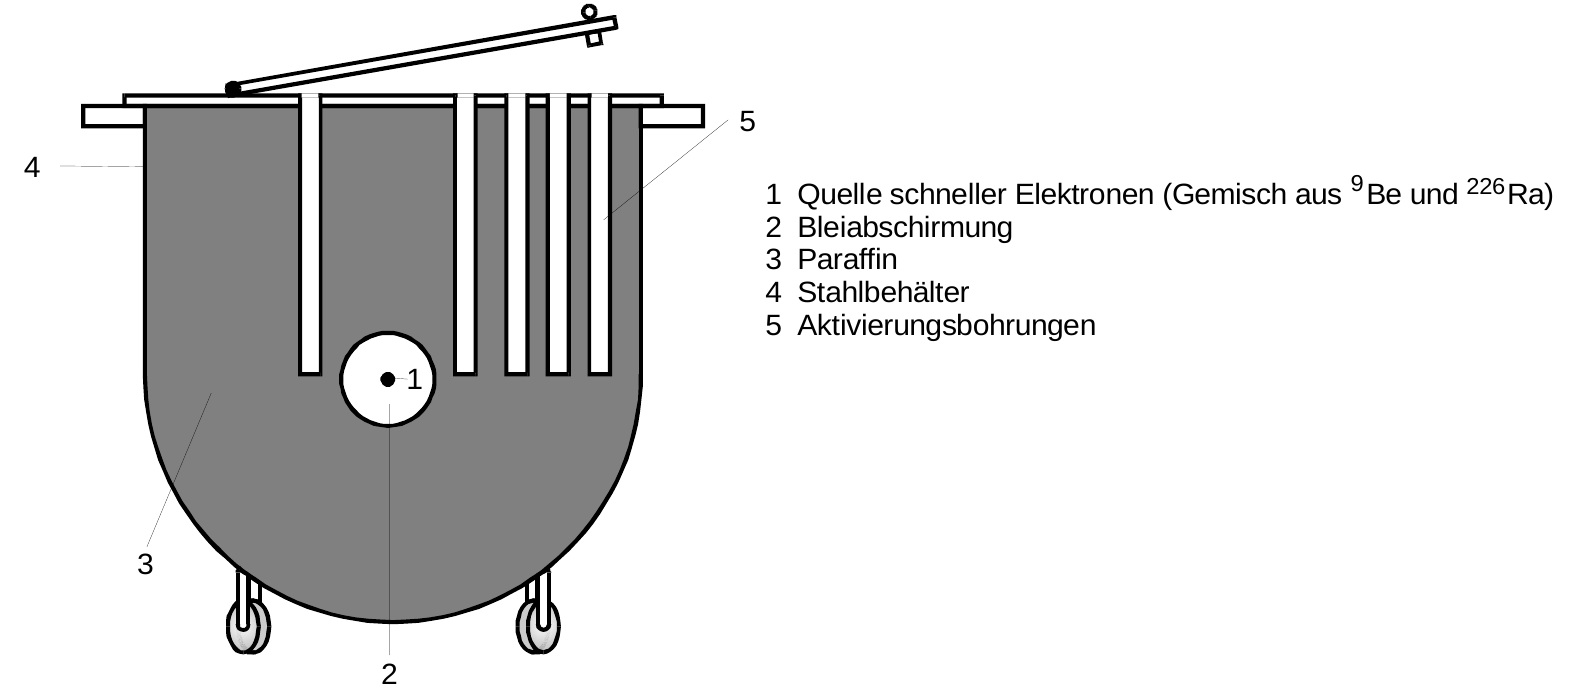
\includegraphics[scale=0.4]{pictures/Neutronen.png}
    \caption{Skizze der Neutronenquelle. \cite{AP04}}
    \label{fig:Kessel}
  \end{figure}
\noindent
Und diesen Messen wir dann einfach mit einem Geiger-Müller 
Zählrohr und schirmen die Quelle und das Zählrohr zur Sicherheit mit Blei ab. Ich zeiche das mal nur sehr grob. Dann wird das Signal von
einem Verstärker noch verstärkt und wird an zwei Zähler weiter geleitet. Dazwischen ist dann ein Schalter, der immer zwischen den beiden Zählern
hin und her schaltet, sodass wir die Zählrate bequem ablesen können (Abb.\ref{fig:Apparatur}). 
\begin{figure}[H]
    \centering
    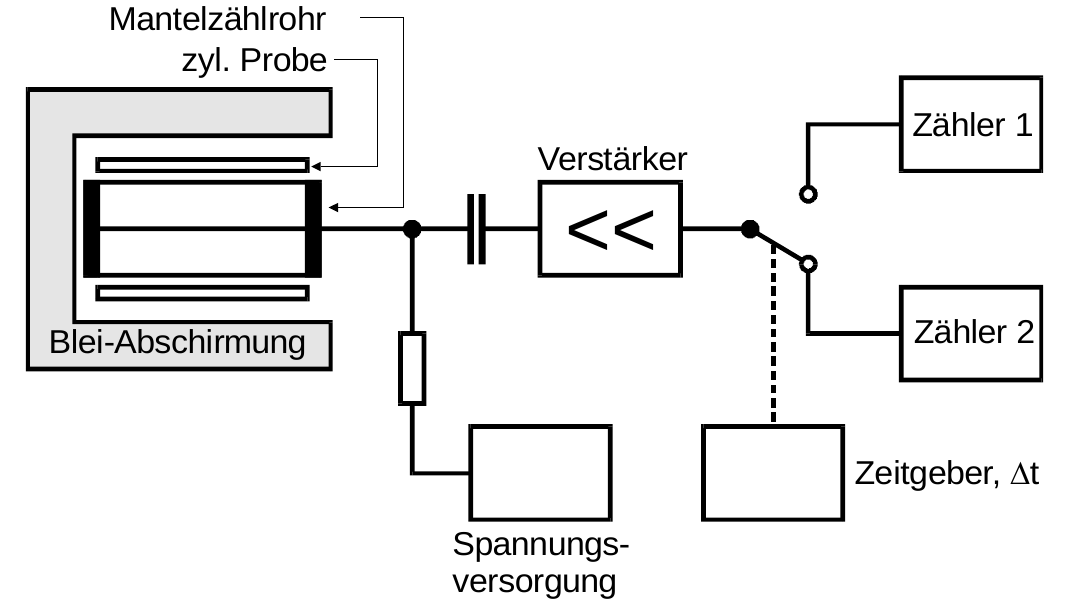
\includegraphics[scale=0.4]{pictures/Messapparatur.png}
    \caption{Skizze der Messapparatur. \cite{AP04}}
    \label{fig:Apparatur}
  \end{figure}
\noindent
Den radioaktiven Zerfall beschreiben wir dann mathematisch über das Zerfallsgesetz. 
\\\\\noindent
\textit{Dann schreiben Sie mal an, wie das aussieht.}
\\\\\noindent
\begin{equation}
    N(t)=N_0\exp(-\gamma t)
\end{equation}
mit der Zerfallskonstante $\gamma$.
\begin{figure}[H]
    \centering
    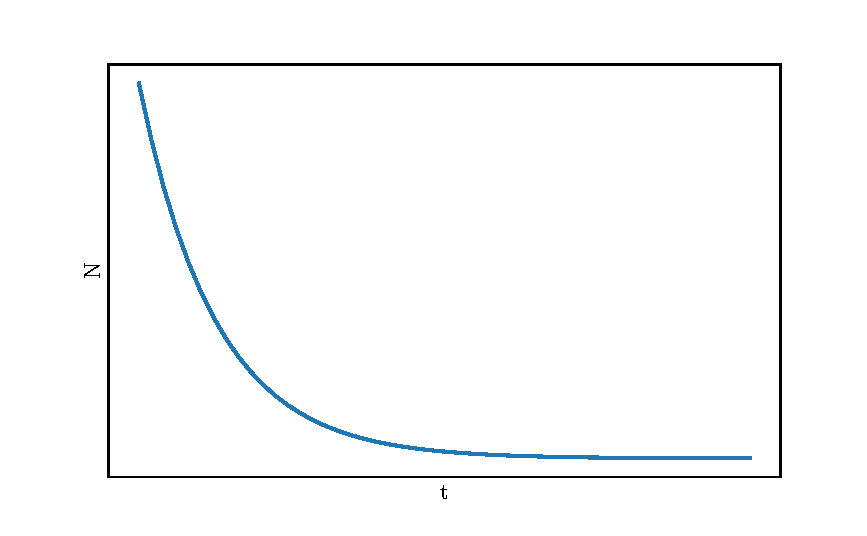
\includegraphics[scale=0.8]{pictures/Zerfallsgesetz.pdf}
    \caption{Verlauf des Zerfallgesetztes}
    \label{fig:Zerfall}
  \end{figure}
\noindent
\textit{Man misst ja bei dem Versuch eine Zählrate. Wie berechnen sich denn die Unsicherheiten?}
\\\\\noindent
Die Unsicherheit erhält man einfach durch Wurzelziehen
\begin{equation}
    \Delta N=\sqrt{N}
\end{equation}
Sie sind also Poission verteilt.
\\\\\noindent
Mit dem Zerfallsgesetz kann man sich jetzt auch noch eine sehr wichtige Größe definieren, um den Radioaktiven Zerfall zu beschreiben, nämlich
die Halbwertszeit. Die beschriebt wie lange es dauert, bis die Hälfte eines Materials zerfallen ist. Also muss man bei dem Zerfallsgesetz 
einfach nur ein $1/2$ vor schreiben und die Zeit durch die Halbwertszeit ersetzten. Es ist auch sehr interessant, in welchen Größenordnungen 
die Halbwertszeit verteilt ist. Je nach Isotop können das einige Sekunden oder auch viele Millionen Jahre sein. Bei dem Vanadium-Isotop liegt
die Halbwertszeit im Bereich einigen Sekunden und bei $\ce{^{104}Rh}$ bei wenigen Minuten.
\\\\\noindent
\textit{Sonst würde man ja auch ganz schön lange messen.}
\\\\\noindent
Wir haben den Versuch ja nicht wirklich durchgeführt, von daher war jeder Messzeitraum recht bequem für uns.
\\\\\noindent
(Frau Siegmann erzählte, dass sie die Messdaten ja aufgenommen hat und recht froh war, nicht monatelang messen zu müssen.)
\\\\\noindent
Jetzt haben wir bei Rhodium ja diesen Besonderen Fall, dass wir zwei Zerfälle gleichzeitig haben. Um die Halbwertszeiten von den beiden 
Isotopen zu bestimmen hilft es aber zu wissen, dass die Halbwertszeit von $\ce{^{104i}Rh}$ deutlich kürzer ist als die von 
$\ce{^{104}Rh}$. Also muss man nur eine Zeit warten, dann ist der Betrag von $\ce{^{104i}Rh}$ zu vernachlässigen und man kann die 
Halbwertszeit von $\ce{^{104}Rh}$ bestimmen. Und wenn man die dann kennt, kann man auch auf die von $\ce{^{104i}Rh}$ zurückrechnen. 
\\\\\noindent
\textit{Wir haben mal einen Gürtel auf sein Alter untersucht, idem wir die Stahlung gemessen haben.}
\\\\\noindent
Das lief bestimmt über das radioaktive Kohlenstoffisotop, was sehr regelmäßig durch kosmische Strahlung in der Atmosphäre ensteht. Und 
dann kann man messen wie stark die Stahlung ist, wie viel also schon zerfallen ist. 
\\\\\noindent
\textit{Ja und wegen der hohen Halbwertszeit kann damit das Alter von archiologischen Funden bestimmt werden.}
\\\\\noindent
(Danach wollte ich dann noch was über die Messung mit dem Geiger Müller Zählrohr erzählen, wurde dann aber schon vor die Tür geschickt,
da meine Prüfungszeit mit ca.25 Minuten schon beendet war.)

\section{Feedback und Note}
Die Prüfer schienen sehr zufreiden mit der Prüfung gewesen zu sein und bewerteten die Prüfung deswegen mit 1.0. Frau Siegmann wies auch noch
einmal explizit darauf hin, dass sie es gut findet, dass ich auch die online Versuche gut gelernt habe. 

\section{Anmerkungen}
Ich empfand die Atmosphäre der Prüfung als sehr offen und freundlich. Die Prüfer haben regelmäßig durch Nicken oder ihre Mimik Feedback gegeben,
ob das, was ich erzähle, in die richtige Richtung geht. Besonders angenehm fand ich die Tatsache, dass mein Vorschlag für den zweiten 
Versuch auch angenommen wurde. Ich hatte generell das Gefühl, dass ich selbst recht gut lenken konnte, in welche Richtung
sich die Prüfung entwickelt.
\\\noindent
Das Gedächtnisprotokoll habe ich direkt nach der Prüfung erstellt, der genaue Wortlaut kann natürlich trotzdem nicht zu $\SI{100}{\percent}$
reproduziert werden.
